\documentclass{beamer}
\usepackage{graphicx}
\graphicspath{ {images/} }

\usepackage{default}

\begin{document}
	\title{One Chain, Two Chain, Three Chain, More?}
	\subtitle{A Monte Carlo Study}
	\author{Zack Roman}
	\institute{University of Kansas}
	\date{\today}
	
\begin{frame}
	
	\titlepage
	
\end{frame}

\begin{frame}
	\frametitle{Outline}
	\tableofcontents
\end{frame}



\section{Method}
\subsection{Data Generation}

\begin{frame}
\frametitle{Data Generation}
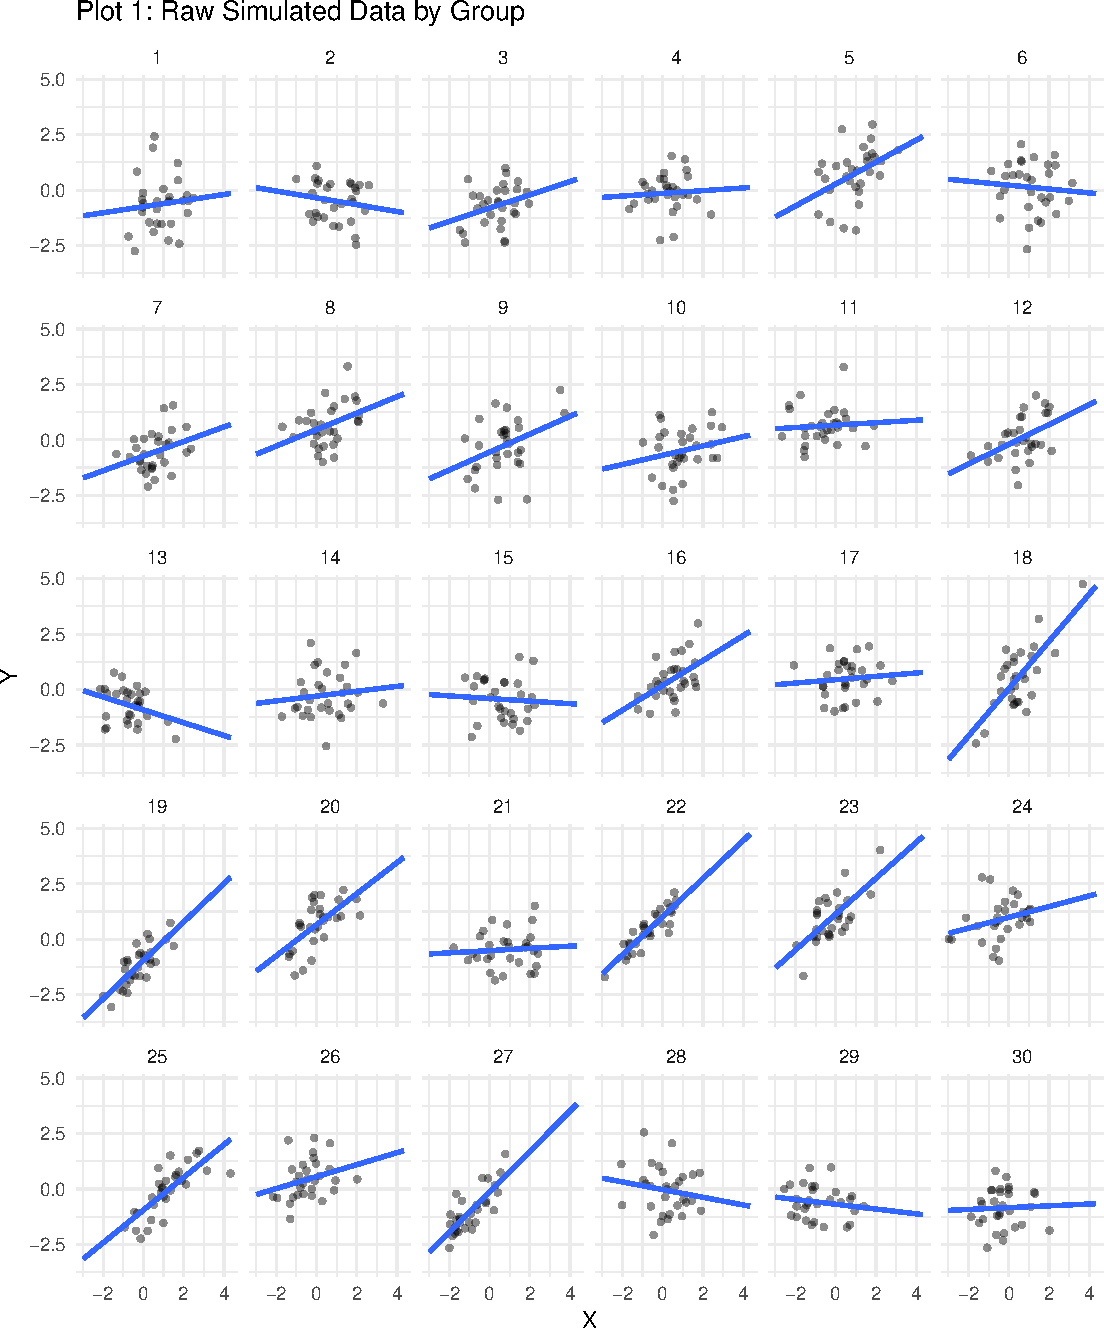
\includegraphics[scale=.35]{Raw_slopes.pdf}
\end{frame}

\begin{frame}
	
\frametitle{Data Generation}
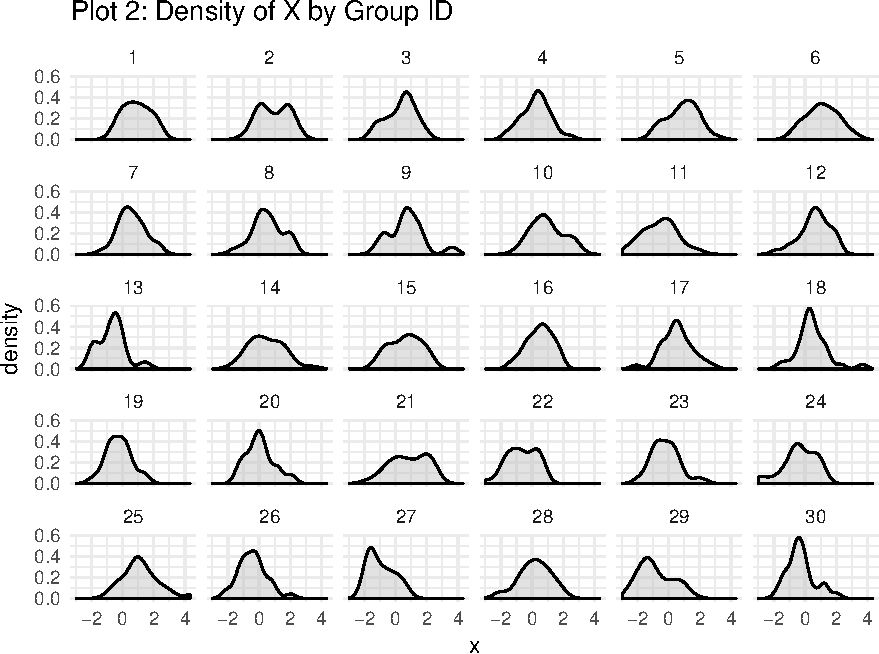
\includegraphics[scale=.75]{Raw_density_x.pdf}

\end{frame}

\begin{frame}
\frametitle{Data Generation}
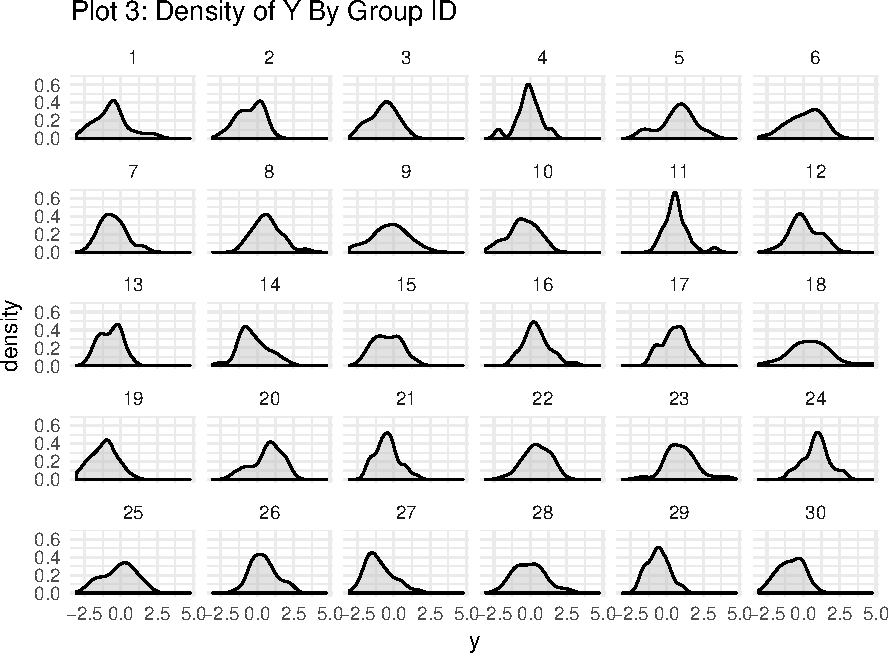
\includegraphics[scale=.75]{Raw_density_y.pdf}
\end{frame}

\subsection{MCMC Analysis}

\begin{frame}
	\frametitle{Prior Conditions}
	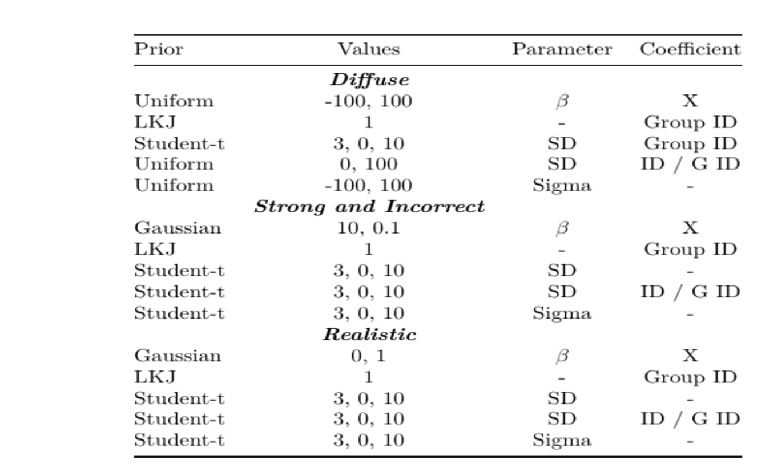
\includegraphics[scale = .75]{prior_table.pdf}
\end{frame}


\begin{frame}
	\frametitle{Results and Convergence: Realistic}
	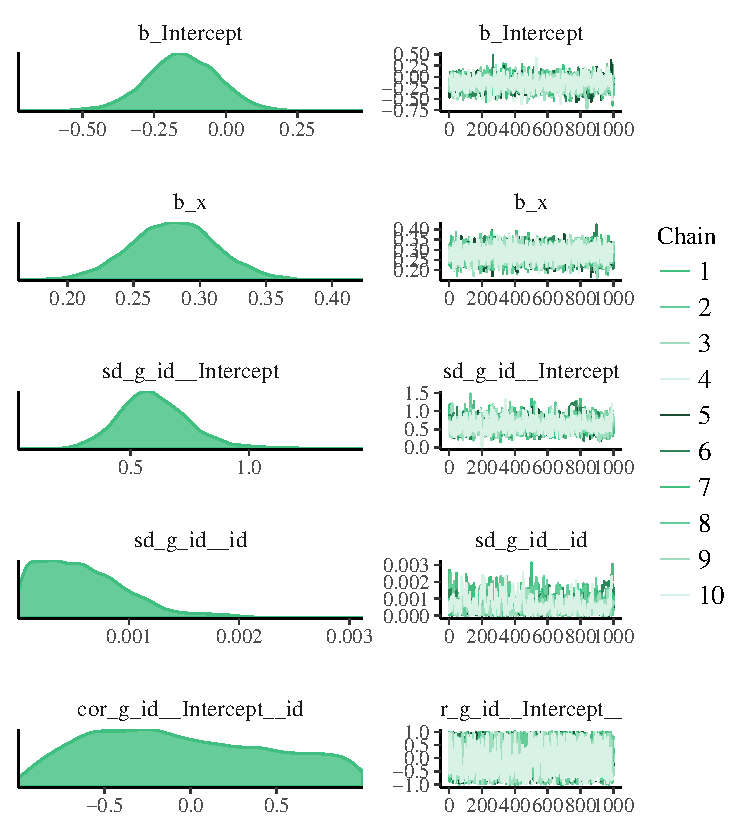
\includegraphics[scale=.5]{str_cor_fit.pdf}
\end{frame}

\begin{frame}
\frametitle{Results and Convergence: Diffuse}
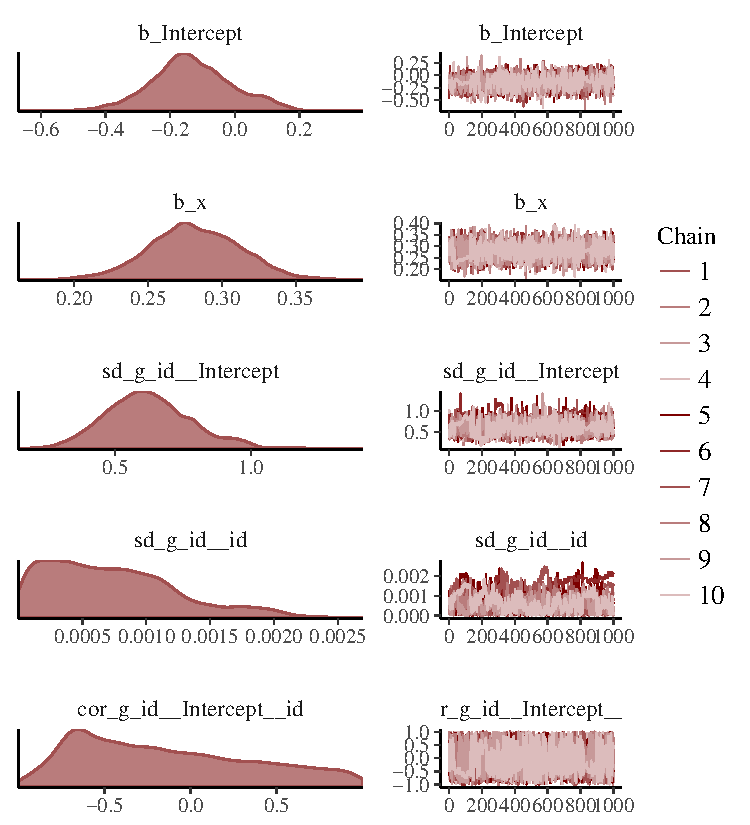
\includegraphics[scale=.5]{dif_fit.pdf}
\end{frame}

\begin{frame}
	\frametitle{Results and Convergence: Strong and Incorrect}
	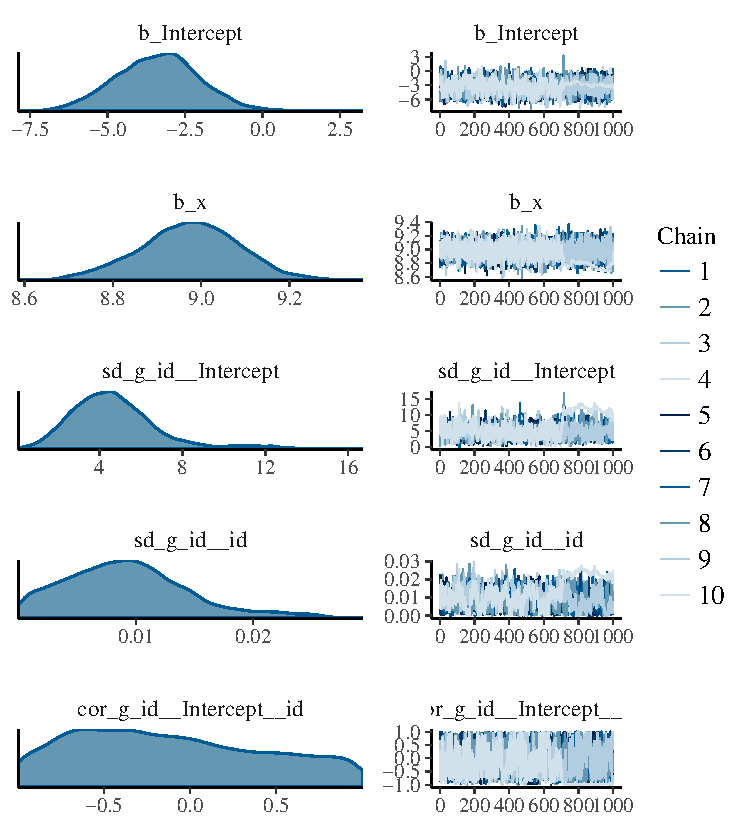
\includegraphics[scale=.5]{str_inc_fit.pdf}
\end{frame}

\subsection{Sampling of Chains}

\begin{frame}
	\frametitle{Sampling of Chains}
\begin{itemize}
	\item Chains sampled without replacement
	\item 2 through 9 chain conditions
	\item 1,000 itterations of sampling per chain
	\item Total Number of Conditions: 8*3 = 24
\end{itemize}
\end{frame}


\section{Results}
\subsection{Convergence}
\begin{frame}
	\frametitle{Convergence}
	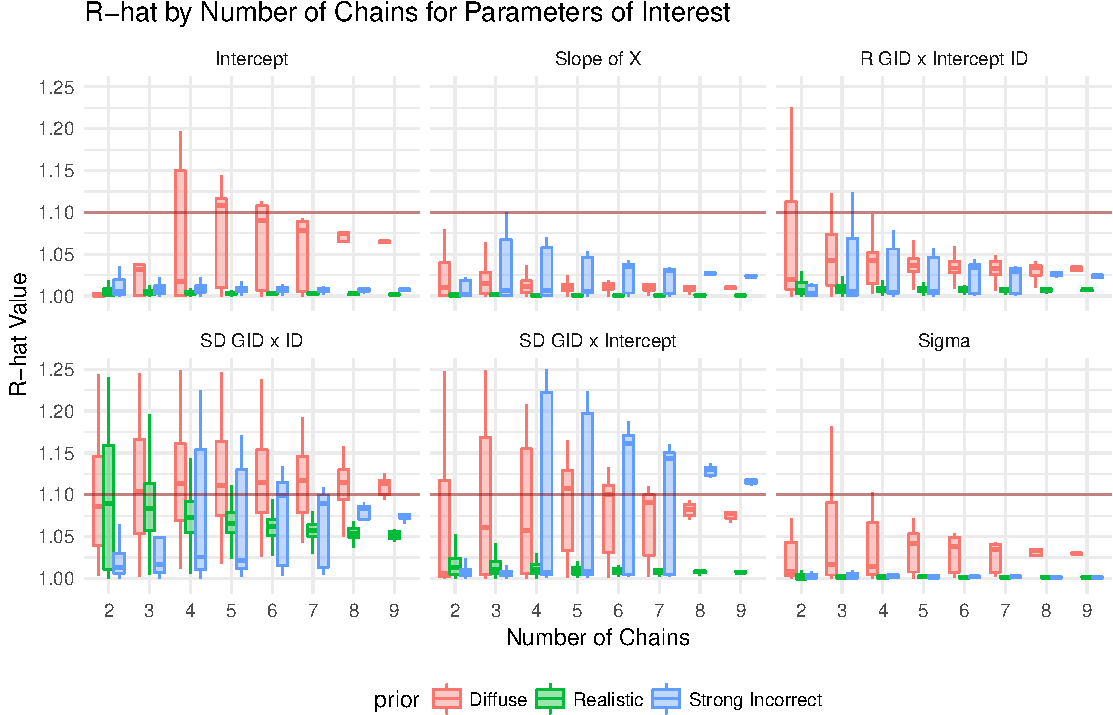
\includegraphics[scale=.57]{convergence_parm.pdf}
\end{frame}

\begin{frame}
	\frametitle{Convergence}
	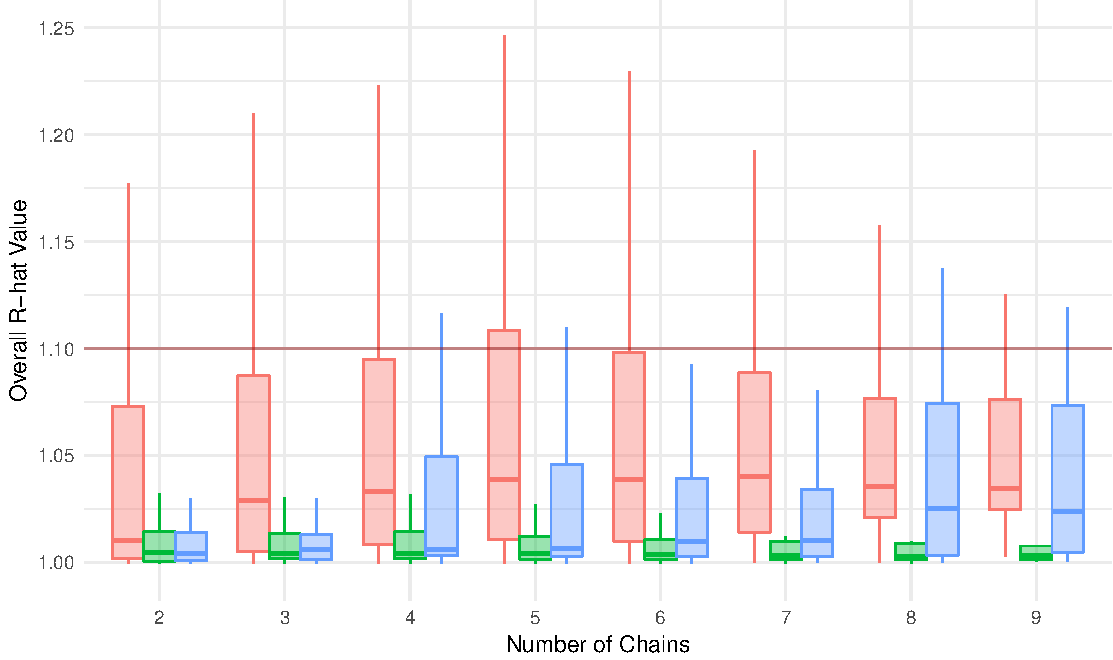
\includegraphics[scale=.57]{convergence.pdf}
\end{frame}

\begin{frame}
	\frametitle{Convergence}
	\begin{center}
	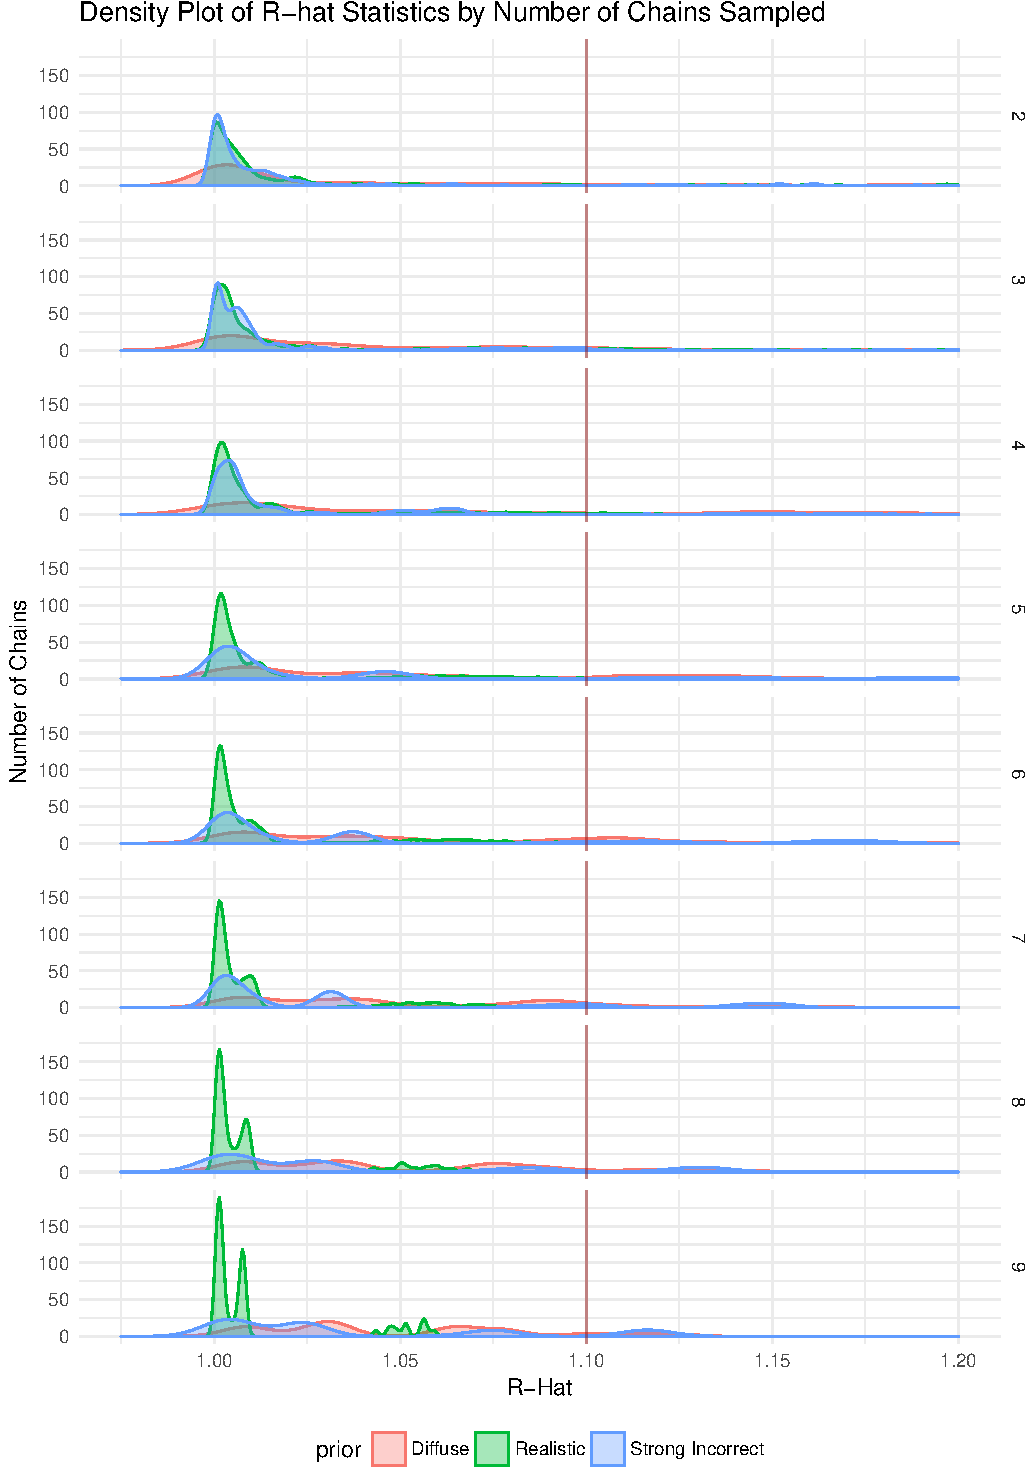
\includegraphics[scale=.30]{denisty_convergence.pdf}
	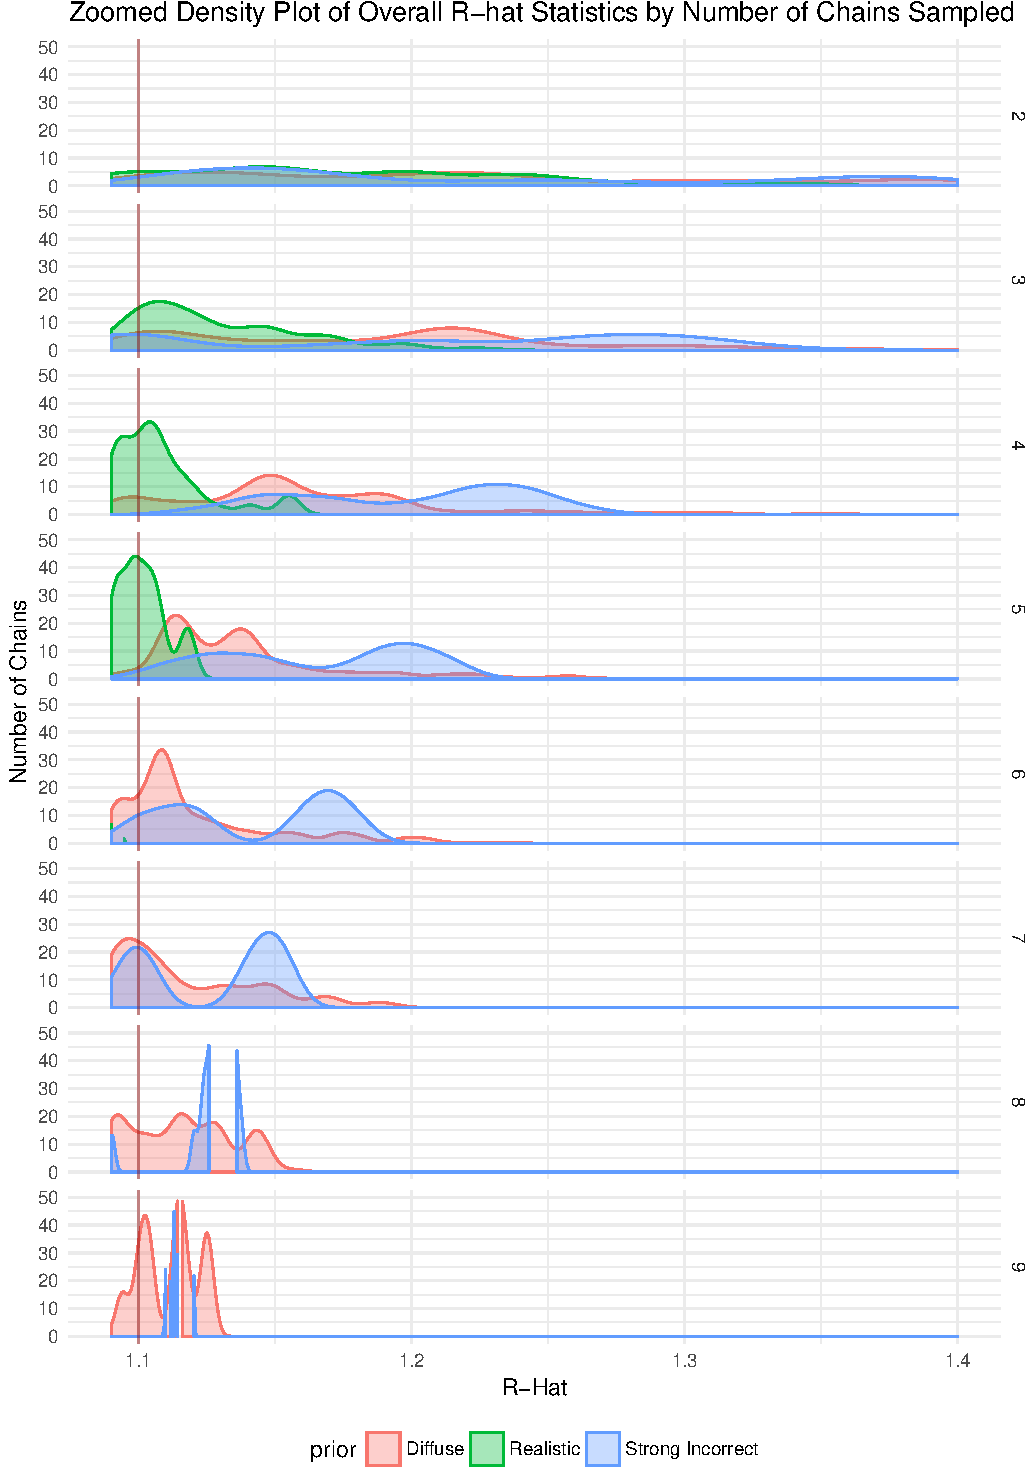
\includegraphics[scale=.30]{zoomed_denisity_convergence.pdf}
	\end{center}
\end{frame}


\subsection{Bias}

\begin{frame}
	\frametitle{Bias}
	\begin{center}
	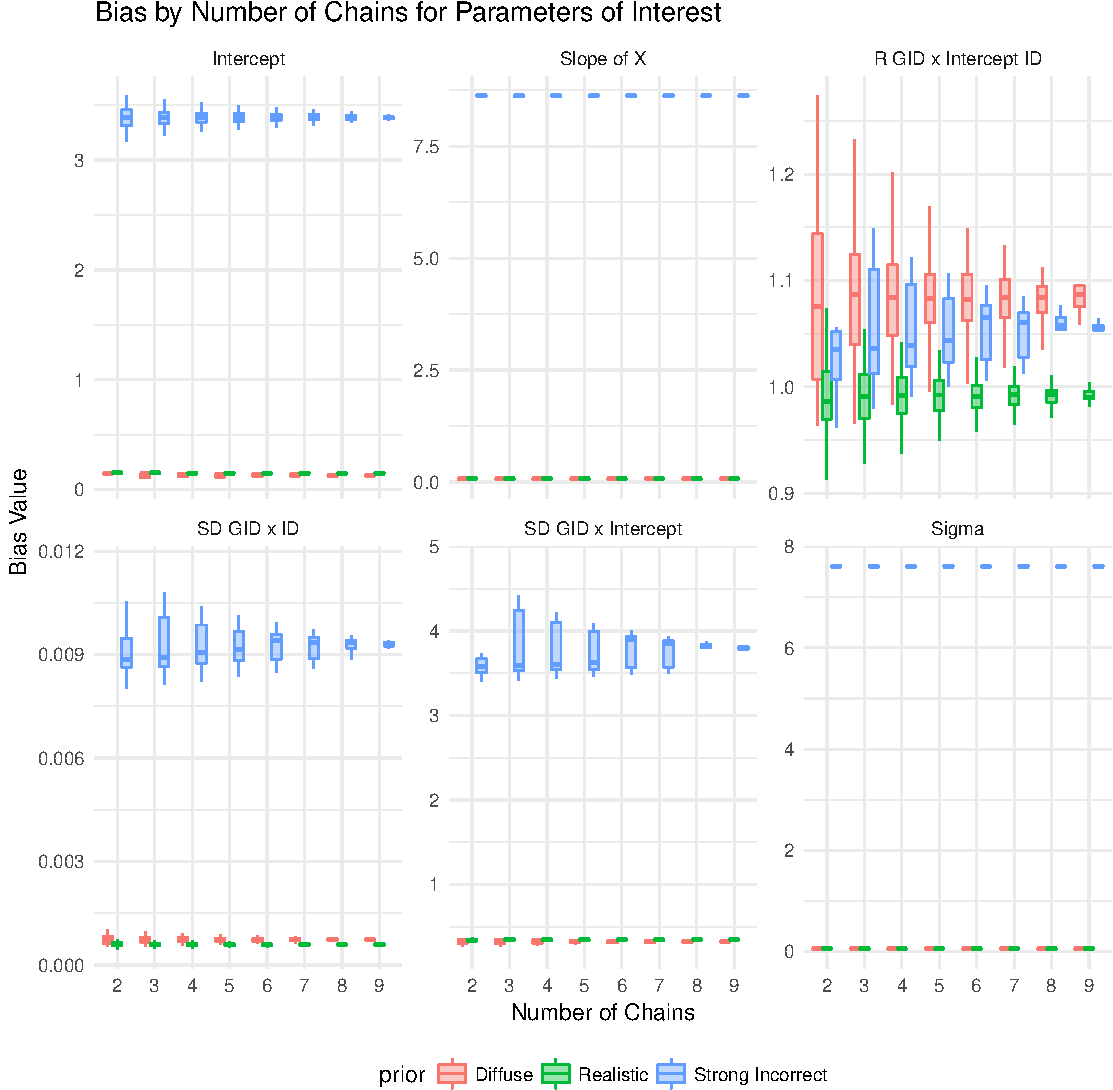
\includegraphics[scale=.45]{Box_bias.pdf}
	\end{center}
\end{frame}


\begin{frame}
	\frametitle{Bias}
	\begin{center}
		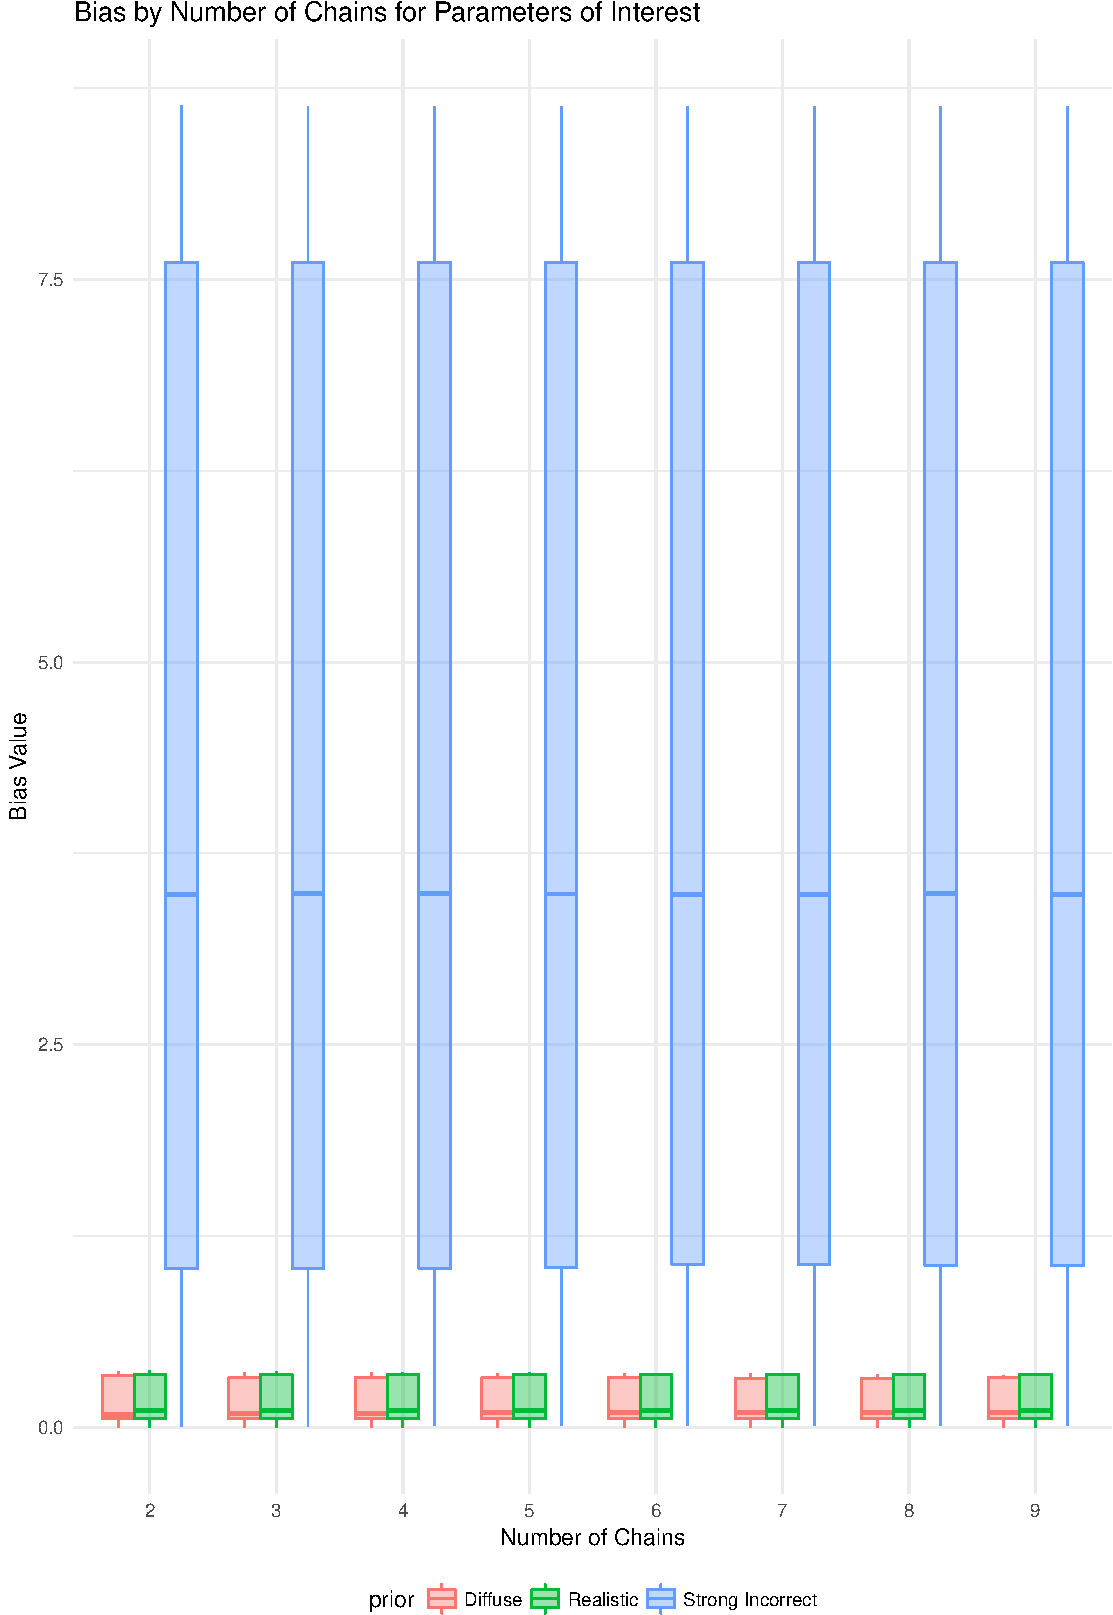
\includegraphics[scale=.30]{full_box_bias.pdf}
	\end{center}
\end{frame}



\subsection{Convergence and Bias}

\begin{frame}
	\frametitle{Relationship: Convergence and Bias}
	\begin{center}
		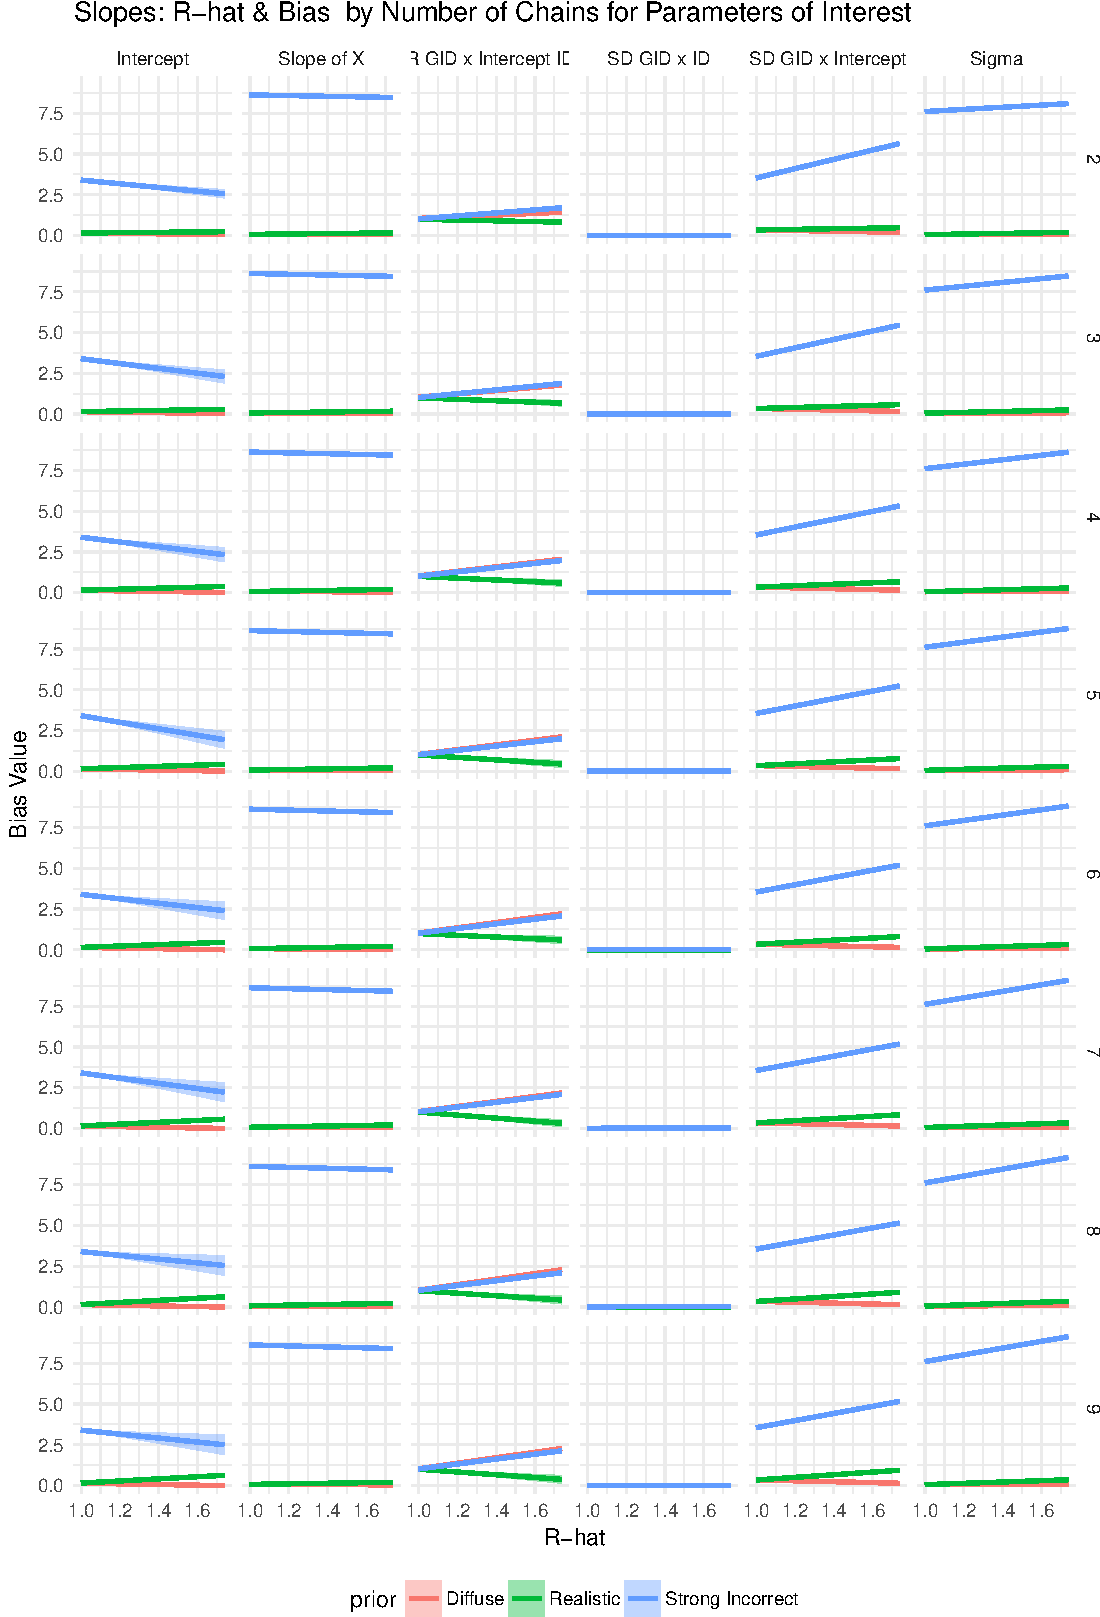
\includegraphics[scale=.30]{Slopes.pdf}
	\end{center}
\end{frame}

\begin{frame}
	\frametitle{Relationship: Convergence and Bias}
	\begin{center}

		\includegraphics[scale = 1]{cor_tab.pdf}

	\end{center}
\end{frame}






\end{document}
